\documentclass{standalone}
\usepackage{standalone}
\usepackage{tikz}
\usepackage{graphicx}
\usepackage{float}
\usepackage{listings}
\usepackage{caption}
\usepackage{fancyhdr}
\begin{document}
% \begin{framed}
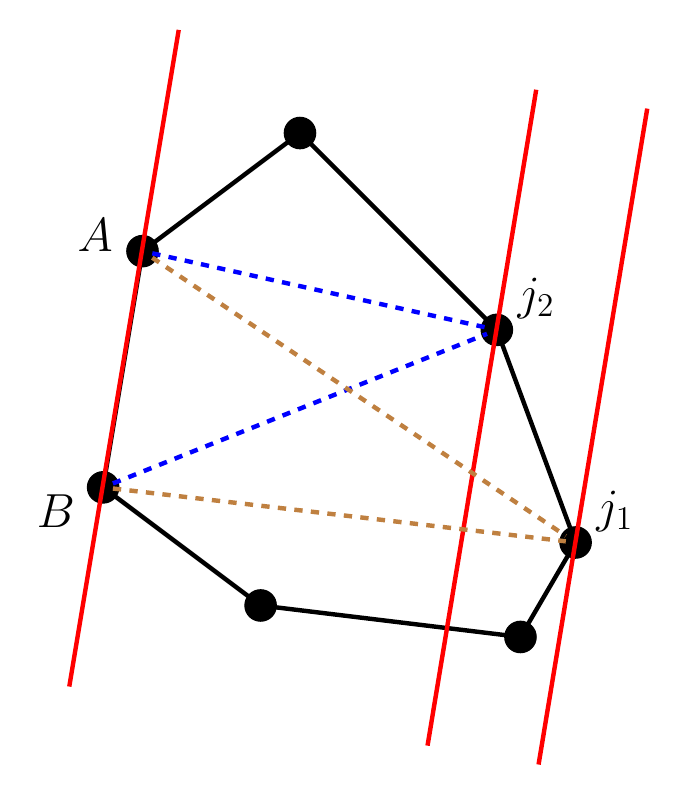
\begin{tikzpicture}
\node (a) at (1.5, 7) {};
\node (b) at (1, 4) {};
\node (c) at (3, 2.5) {};
\node (d) at (6.3, 2.1) {};
\node (e) at (7, 3.3) {};
\node (f) at (6, 6) {};
\node (g) at (3.5,8.5) {};

\filldraw (a) circle (.2) (b) circle (.2) (c) circle (.2) (d) circle (.2) (e) circle (.2) (f) circle (.2) (g) circle (.2) ;
\draw[ultra thick] (a)--(b) (b)--(c) (c)--(d) (d)--(e) (e)--(f) (f)--(g) (g)--(a);
\draw[ultra thick,color = red] (1.96,9.81)--(0.57,1.47) (5.12,0.72)--(6.50,9.05) (6.53,0.48)--(7.91,8.81);
\draw[dashed, ultra thick, color=blue] (a)--(f) (b)--(f);
\draw[dashed, ultra thick, color=brown] (a)--(e) (b)--(e);
\node at (0.9, 7.2) [font=\fontsize{17.28}{0}\selectfont] {$A$};
\node at (0.4, 3.7) [font=\fontsize{17.28}{0}\selectfont] {$B$};
\node at (7.5, 3.7) [font=\fontsize{17.28}{0}\selectfont] {$j_1$};
\node at (6.5, 6.4) [font=\fontsize{17.28}{0}\selectfont] {$j_2$};
\end{tikzpicture}
% \end{framed}

\end{document}

Latex Tikz